% TODO change date

%\documentclass[handout,notes]{beamer}
\documentclass[]{beamer}
\usetheme{CambridgeUS}
\usecolortheme{dolphin}
\usepackage{tikz}


\usepackage{pgfpages}

% from here: http://tex.stackexchange.com/questions/151645/how-to-generate-pdf-with-6-slides-from-beamer-presentation
\pgfpagesdeclarelayout{6 on 1}
{
  \edef\pgfpageoptionheight{\the\paperwidth} % landscaped by default
  \edef\pgfpageoptionwidth{\the\paperheight}
  \def\pgfpageoptionborder{0pt}
  \def\pgfpageoptionfirstshipout{1}
}
{
  \pgfpagesphysicalpageoptions
  {%
    logical pages=6,%
    physical height=\pgfpageoptionheight,%
    physical width=\pgfpageoptionwidth,%
    current logical shipout=\pgfpageoptionfirstshipout%
  }
  \ifdim\paperheight>\paperwidth\relax
    % put side-by-side
    \pgfpageslogicalpageoptions{1}
    {%
      border shrink=\pgfpageoptionborder,%
      resized width=.5\pgfphysicalwidth,%
      resized height=\pgfphysicalheight,%
      center=\pgfpoint{.1667\pgfphysicalwidth}{.25\pgfphysicalheight}%
    }%
    \pgfpageslogicalpageoptions{3}
    {%
      border shrink=\pgfpageoptionborder,%
      resized width=.5\pgfphysicalwidth,%
      resized height=\pgfphysicalheight,%
      center=\pgfpoint{.5\pgfphysicalwidth}{.25\pgfphysicalheight}%
    }%
    \pgfpageslogicalpageoptions{5}
    {%
      border shrink=\pgfpageoptionborder,%
      resized width=.5\pgfphysicalwidth,%
      resized height=\pgfphysicalheight,%
      center=\pgfpoint{.8333\pgfphysicalwidth}{.25\pgfphysicalheight}%
    }%
    \pgfpageslogicalpageoptions{2}
    {%
      border shrink=\pgfpageoptionborder,%
      resized width=.5\pgfphysicalwidth,%
      resized height=\pgfphysicalheight,%
      center=\pgfpoint{.1667\pgfphysicalwidth}{.75\pgfphysicalheight}%
    }%
    \pgfpageslogicalpageoptions{4}
    {%
      border shrink=\pgfpageoptionborder,%
      resized width=.5\pgfphysicalwidth,%
      resized height=\pgfphysicalheight,%
      center=\pgfpoint{.5\pgfphysicalwidth}{.75\pgfphysicalheight}%
    }%
    \pgfpageslogicalpageoptions{6}
    {%
      border shrink=\pgfpageoptionborder,%
      resized width=.5\pgfphysicalwidth,%
      resized height=\pgfphysicalheight,%
      center=\pgfpoint{.8333\pgfphysicalwidth}{.75\pgfphysicalheight}%
    }%
  \else
    % stack on top of one another
    \pgfpageslogicalpageoptions{1}
    {%
      border shrink=\pgfpageoptionborder,%
      resized width=0.5\pgfphysicalwidth,%
      resized height=\pgfphysicalheight,%
      center=\pgfpoint{.25\pgfphysicalwidth}{.8333\pgfphysicalheight}%
    }%
    \pgfpageslogicalpageoptions{3}
    {%
      border shrink=\pgfpageoptionborder,%
      resized width=0.5\pgfphysicalwidth,%
      resized height=\pgfphysicalheight,%
      center=\pgfpoint{.25\pgfphysicalwidth}{.5\pgfphysicalheight}%
    }%
    \pgfpageslogicalpageoptions{5}
    {%
      border shrink=\pgfpageoptionborder,%
      resized width=0.5\pgfphysicalwidth,%
      resized height=\pgfphysicalheight,%
      center=\pgfpoint{.25\pgfphysicalwidth}{.1667\pgfphysicalheight}%
    }%
    \pgfpageslogicalpageoptions{2}
    {%
      border shrink=\pgfpageoptionborder,%
      resized width=0.5\pgfphysicalwidth,%
      resized height=\pgfphysicalheight,%
      center=\pgfpoint{.75\pgfphysicalwidth}{.8333\pgfphysicalheight}%
    }%
    \pgfpageslogicalpageoptions{4}
    {%
      border shrink=\pgfpageoptionborder,%
      resized width=0.5\pgfphysicalwidth,%
      resized height=\pgfphysicalheight,%
      center=\pgfpoint{.75\pgfphysicalwidth}{.5\pgfphysicalheight}%
    }%
    \pgfpageslogicalpageoptions{6}
    {%
      border shrink=\pgfpageoptionborder,%
      resized width=0.5\pgfphysicalwidth,%
      resized height=\pgfphysicalheight,%
      center=\pgfpoint{.75\pgfphysicalwidth}{.1667\pgfphysicalheight}%
    }%
  \fi
}

\mode<handout>{
    \pgfpagesuselayout{6 on 1}[letterpaper, border shrink=8mm]
    \pgfpageslogicalpageoptions{1}{border code=\pgfusepath{stroke}}
    \pgfpageslogicalpageoptions{2}{border code=\pgfusepath{stroke}}
    \pgfpageslogicalpageoptions{3}{border code=\pgfusepath{stroke}}
    \pgfpageslogicalpageoptions{4}{border code=\pgfusepath{stroke}}
    \pgfpageslogicalpageoptions{5}{border code=\pgfusepath{stroke}}
    \pgfpageslogicalpageoptions{6}{border code=\pgfusepath{stroke}}
}
\newcommand{\vocab}[1]{\textcolor{blue}{\textbf{#1}}}

%\usepackage{beamerthemesplit} % Activate for custom appearance

\title{Rigiditea}
\author{Rachel Wu, Tony Zhang}
\date{May 10, 2017}

\begin{document}

\frame{\titlepage}

\section[Outline]{}
\frame{\tableofcontents}

\frame{
    \frametitle{Linkage rigidity suite}
    	Our project explores rigidity in 2D linkages
	through a GUI-based web application.
	In particular, we
	
	\begin{enumerate}
	    \item created an interface for designing and manipulating linkages,
	    \item implemented and visualized iterations of the Pebble algorithm,
	    \item and implemented an infinitesimal rigidity tester.
	\end{enumerate}
}

\frame{
    \frametitle{Design goals}
    	In building a web application, we had the following goals in mind.
	
	\begin{enumerate}
	    \item Web interface should be easy to use and understand,
	    especially for users unfamiliar with linkages.
	    \item Algorithms should be visualized in an ``intuitive'' way,
	    to facilitate their understanding.
	    \item Try out CoffeeScript! (and polish up on \texttt{d3.js}?)
	\end{enumerate}
}

\section{Interface}

\frame{
    \frametitle{GUI interface}
    Our user interface has several features. Users are currently able to
    
    \begin{enumerate}
    	\item design graphs by clicking and dragging, and
	\item step through the Pebble algorithm,
	one iteration at a time.
    \end{enumerate}
    \begin{center}
    	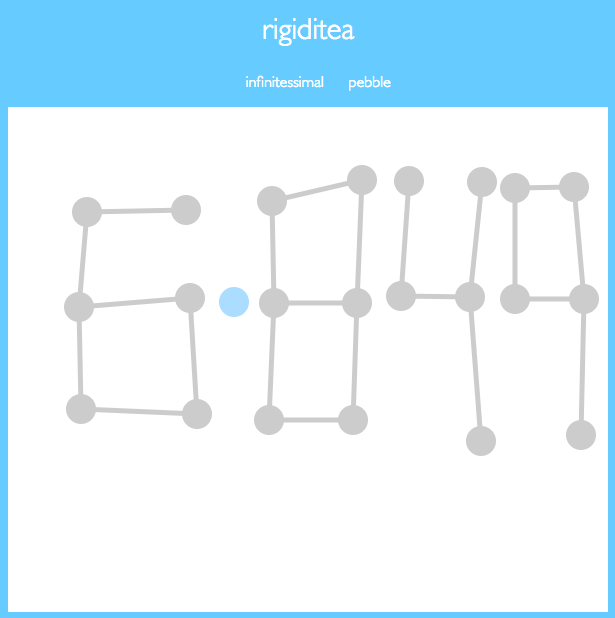
\includegraphics[scale=.2]{fig/fig-gui-basic}
    \end{center}

    In the near future, we will add infinitesimal rigidity visualization,
    whose backend has already been written.
}

\frame{
    \frametitle{Underlying linkage representation}
    \begin{itemize}
    \item We represent linkages as \texttt{PebbleGraph} objects,
    or undirected graphs in adjacency list form.
    \item Each graph has vertices and edges,
    which carry their own attributes (e.g. number of pebbles)
    \end{itemize}
}


\section{The pebble game}

\frame{
    \frametitle{Conditions for rigidity}
    
}

\frame{
    \frametitle{The game}
    \begin{itemize}
        \item
        Given undirected graph $G = (V, E)$,
        give two pebbles to each vertex.
        Each vertex can use its pebbles to cover incident edges.
        \item
        A \vocab{pebble covering} is an assignment of pebbles
        such that each edge is covered by a pebble.
        \item
        
    \end{itemize}
}

\section{Extensions}

\begin{frame}
    \frametitle{Work yet to be completed}
    There are several items we plan to complete.
    \begin{enumerate}
        \item Smooth out the GUI with animations
        and possibly, user-friendly keyboard shortcuts.
        \item Introduce more granularity in each ``step'' of the Pebble algorithm.
        \item Animate or visualize infinitesimal rigidity results on the graph as well.
    \end{enumerate}
    In general, we plan to improve the GUI for a user-friendly and intuitive experience.
\end{frame}



\begin{frame}
  \frametitle{Further Reading}
  \begin{thebibliography}{10}
  \beamertemplatebookbibitems
  \bibitem{pebble}
  Donald J. Jacobs, Bruce Hendrickson, An Algorithm for Two-Dimensional Rigidity Percolation: The Pebble Game, \textit{J.~Comp.~Phys.} 137, 346-365 (1997)
  \end{thebibliography}
\end{frame}

\end{document}
